\documentclass[conference]{IEEEtran}
\IEEEoverridecommandlockouts
% The preceding line is only needed to identify funding in the first footnote. If that is unneeded, please comment it out.
\usepackage[nocompress]{cite}
\usepackage{amsmath,amssymb,amsfonts}
\usepackage{algorithmic}
\usepackage{graphicx}
\usepackage{textcomp}
\usepackage{xcolor}

\usepackage{ngerman}
\usepackage[utf8]{inputenc}
\usepackage{longtable}
\usepackage{float}
%\usepackage[breaklinks]{hyperref}
\usepackage{url}

\def\BibTeX{{\rm B\kern-.05em{\sc i\kern-.025em b}\kern-.08em
		T\kern-.1667em\lower.7ex\hbox{E}\kern-.125emX}}
\begin{document}
	
	\title{Multilinguale Spracherkennung mit tiefen neuronalen
	Netzen\\
	}
	
	\author{\IEEEauthorblockN{1\textsuperscript{st} Björn Beha}
		\IEEEauthorblockA{\textit{dept. name of organization (of Aff.)} \\
			\textit{name of organization (of Aff.)}\\
			City, Country \\
			email address}
		\and
		\IEEEauthorblockN{2\textsuperscript{nd} Philipp Ginter}
		\IEEEauthorblockA{\textit{dept. name of organization (of Aff.)} \\
			\textit{name of organization (of Aff.)}\\
			City, Country \\
			email address}
		\and
		\IEEEauthorblockN{3\textsuperscript{rd} Suhay Sevinc}
		\IEEEauthorblockA{\textit{dept. name of organization (of Aff.)} \\
			\textit{name of organization (of Aff.)}\\
			City, Country \\
			email address}
	}
	
	\maketitle
	
	\begin{abstract}
	Dieser Artikel beschäftigt sich mit dem Ansatz des tiefen maschinellen Lernens im Bereich der multilingualen Spracherkennung.	Die Arbeit setzt sich mit der Forschungsfrage auseinander, welches Verfahren heute genutzt wird, um aktuelle Spracherkennungssysteme zu realisieren. Aus dieser Untersuchung geht hervor, dass die Genauigkeit der heutigen Spracherkennung über Long short-term memory-Netzwerke erreicht wird, die sich an vorherige Ereignisse erinnern können. Die Arbeit zeigt, warum diese Art von neuronalen Netzen ideal für Sequenzen von Tönen geeignet ist. In diesem Kontext wird untersucht, wie die Erkennung mehrerer Sprachen funktioniert, auch wenn nur geringe Mengen an Trainingsdaten verfügbar sind. Vor allem diese Knappheit von Ressourcen stellt eine Herausforderung dar, da ohne eine Menge von markierten Datensätzen keine Muster und Gesetzmäßigkeiten der Sprache erkannt und beurteilt werden können. Die Abhandlung zeigt, dass dies über das gemeinsame Nutzen einzelner Töne gelöst wird und wie sich ein solches System trainieren lässt. Weiterhin bestehende Herausforderungen werden diskutiert und es wird geklärt, welche Ansätze man in Zukunft verfolgt, um eine natürliche Interaktion zwischen Mensch und Maschine zu ermöglichen.
	\end{abstract}
	
	\begin{IEEEkeywords}
		Tiefes Lernen, tiefe neuronale Netze, Spracherkennung, Recurrent Neural Netzworks, Long short-term memory, LSTM 
	\end{IEEEkeywords}
	

	
	%
% paper title
% Titles are generally capitalized except for words such as a, an, and, as,
% at, but, by, for, in, nor, of, on, or, the, to and up, which are usually
% not capitalized unless they are the first or last word of the title.
% Linebreaks \\ can be used within to get better formatting as desired.
% Do not put math or special symbols in the title.
\title{MicroProfile \\ {\large Optimizing Enterprise Java for a microservices architecture}}
%
%
% author names and IEEE memberships
% note positions of commas and nonbreaking spaces ( ~ ) LaTeX will not break
% a structure at a ~ so this keeps an author's name from being broken across
% two lines.
% use \thanks{} to gain access to the first footnote area
% a separate \thanks must be used for each paragraph as LaTeX2e's \thanks
% was not built to handle multiple paragraphs
%
%
%\IEEEcompsocitemizethanks is a special \thanks that produces the bulleted
% lists the Computer Society journals use for "first footnote" author
% affiliations. Use \IEEEcompsocthanksitem which works much like \item
% for each affiliation group. When not in compsoc mode,
% \IEEEcompsocitemizethanks becomes like \thanks and
% \IEEEcompsocthanksitem becomes a line break with idention. This
% facilitates dual compilation, although admittedly the differences in the
% desired content of \author between the different types of papers makes a
% one-size-fits-all approach a daunting prospect. For instance, compsoc 
% journal papers have the author affiliations above the "Manuscript
% received ..."  text while in non-compsoc journals this is reversed. Sigh.

\author{Björn~Beha und Suhay~Sevinc}
% note the % following the last \IEEEmembership and also \thanks - 
% these prevent an unwanted space from occurring between the last author name
% and the end of the author line. i.e., if you had this:
% 
% \author{....lastname \thanks{...} \thanks{...} }
%                     ^------------^------------^----Do not want these spaces!
%
% a space would be appended to the last name and could cause every name on that
% line to be shifted left slightly. This is one of those "LaTeX things". For
% instance, "\textbf{A} \textbf{B}" will typeset as "A B" not "AB". To get
% "AB" then you have to do: "\textbf{A}\textbf{B}"
% \thanks is no different in this regard, so shield the last } of each \thanks
% that ends a line with a % and do not let a space in before the next \thanks.
% Spaces after \IEEEmembership other than the last one are OK (and needed) as
% you are supposed to have spaces between the names. For what it is worth,
% this is a minor point as most people would not even notice if the said evil
% space somehow managed to creep in.



% The paper headers
\markboth{Hochschule Furtwangen, 07.02.2018}%
{Shell \MakeLowercase{\textit{et al.}}: Bare Advanced Demo of IEEEtran.cls for IEEE Computer Society Journals}
% The only time the second header will appear is for the odd numbered pages
% after the title page when using the twoside option.
% 
% *** Note that you probably will NOT want to include the author's ***
% *** name in the headers of peer review papers.                   ***
% You can use \ifCLASSOPTIONpeerreview for conditional compilation here if
% you desire.



% The publisher's ID mark at the bottom of the page is less important with
% Computer Society journal papers as those publications place the marks
% outside of the main text columns and, therefore, unlike regular IEEE
% journals, the available text space is not reduced by their presence.
% If you want to put a publisher's ID mark on the page you can do it like
% this:
%\IEEEpubid{0000--0000/00\$00.00~\copyright~2015 IEEE}
% or like this to get the Computer Society new two part style.
%\IEEEpubid{\makebox[\columnwidth]{\hfill 0000--0000/00/\$00.00~\copyright~2015 IEEE}%
%\hspace{\columnsep}\makebox[\columnwidth]{Published by the IEEE Computer Society\hfill}}
% Remember, if you use this you must call \IEEEpubidadjcol in the second
% column for its text to clear the IEEEpubid mark (Computer Society journal
% papers don't need this extra clearance.)



% use for special paper notices
%\IEEEspecialpapernotice{(Invited Paper)}



% for Computer Society papers, we must declare the abstract and index terms
% PRIOR to the title within the \IEEEtitleabstractindextext IEEEtran
% command as these need to go into the title area created by \maketitle.
% As a general rule, do not put math, special symbols or citations
% in the abstract or keywords.


\maketitle

\begin{abstract}
	This document is a model and instructions for \LaTeX.
	This and the IEEEtran.cls file define the components of your paper [title, text, heads, etc.]. *CRITICAL: Do Not Use Symbols, Special Characters, Footnotes, 
	or Math in Paper Title or Abstract.
\end{abstract}



% make the title area
\maketitle


% To allow for easy dual compilation without having to reenter the
% abstract/keywords data, the \IEEEtitleabstractindextext text will
% not be used in maketitle, but will appear (i.e., to be "transported")
% here as \IEEEdisplaynontitleabstractindextext when compsoc mode
% is not selected <OR> if conference mode is selected - because compsoc
% conference papers position the abstract like regular (non-compsoc)
% papers do!
\IEEEdisplaynontitleabstractindextext
% \IEEEdisplaynontitleabstractindextext has no effect when using
% compsoc under a non-conference mode.


% For peer review papers, you can put extra information on the cover
% page as needed:
% \ifCLASSOPTIONpeerreview
% \begin{center} \bfseries EDICS Category: 3-BBND \end{center}
% \fi
%
% For peerreview papers, this IEEEtran command inserts a page break and
% creates the second title. It will be ignored for other modes.
\IEEEpeerreviewmaketitle
	\section{Einführung}\label{sec:introduction}
\IEEEPARstart{S}ysteme zur Spracherkennung finden eine zunehmend größere Verbreitung und Beliebtheit in unserem alltäglichen Leben.
Durch sie gibt es eine weitere Art der Interaktion mit den Geräten.
Das Anwendungsspektrum reicht von sprachgesteuerten Smarthome-Systemen über Smartphones hin zum Einsatz in Autos \cite{Yu.2014}.
Bei weltweit über 7000 gesprochenen Sprachen ist es nur konsequent, multilinguale Spracherkennungssysteme zu entwickeln \cite{Gary.2018}.
Eingesetzt werden diese bei Situationen, in denen die Sprache des Sprechers nicht bekannt ist oder für eine Sprache nur wenig
Trainingsdaten vorhanden sind. In solch einem Fall kann die gemeinsame Nutzung von Phonemen, die fehlenden Daten ausgleichen. [3]

\subsection{Pipeline}
Aus welchen Komponenten und Prozessen besteht ein System zur Spracherkennung?
Traditionelle Systeme mit beispielsweise HMM und GMM, sowie der Einsatz von neuronalen Netzen.
Zu Beginn einer solchen Pipeline steht das analoge Audiosignal, das in ein digitales umgewandelt wird.
Diese Daten werden dann vorverarbeitet. Eine möglicher Schritt ist die Umwandlung in die einzelnen Frequenzen.
In einem Spektrogramm kann man die Daten abbilden – wie es in Abbildung \ref{fig:pipeline} zu sehen ist.
Nach der Vorverarbeitung werden die einzelnen Frequenzen als Features in das

\begin{figure}[h!]
    \centering
    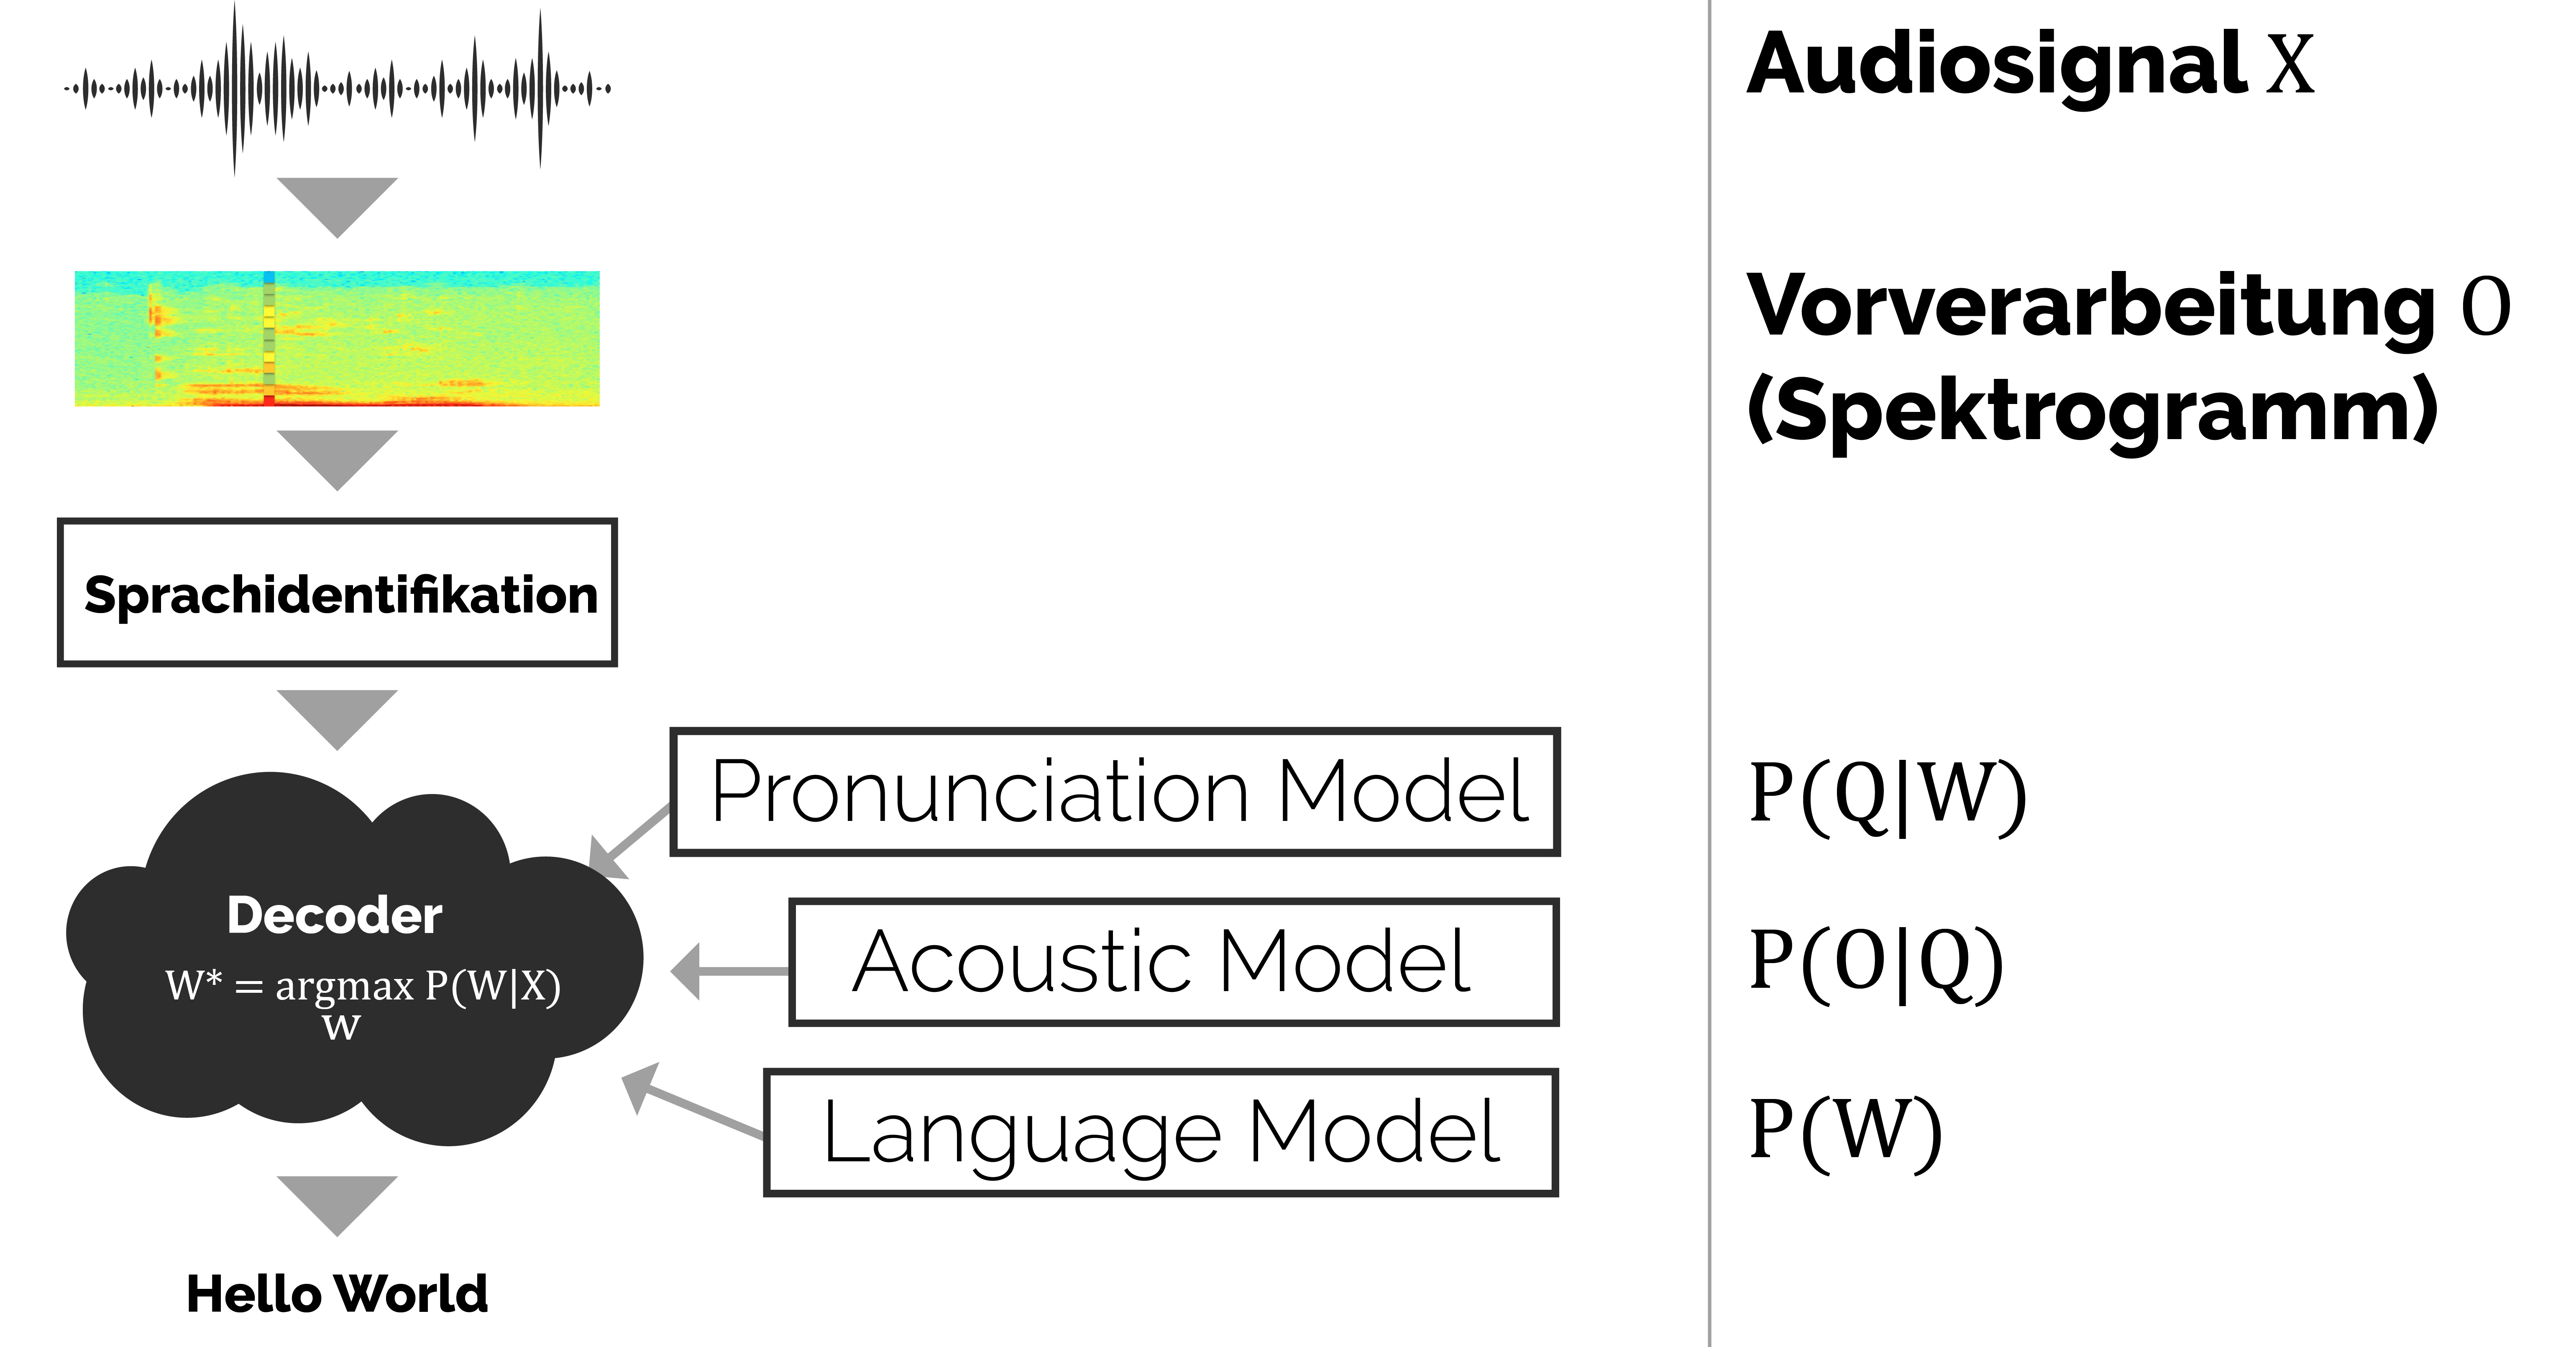
\includegraphics[width=1\linewidth]{images/Presentation-01-01}
    \caption{Pipeline eines Spracherkennungssystems (Nach: ) }%\cite{??}}
    \label{fig:pipeline}
\end{figure}

%Die Arbeit lehnt sich dabei an die von Lars Röwekamp verfassten Artikel auf diversen Plattformen an. Durch seine Beiträge manifestierte er seine grenzenlose Inkompetenz. Scheiß auf dich und dein Copyright.

	\section{Sprachidentifikation}
\subsection{Überblick}
Systeme zur Sprachidentifikation werden eingesetzt um die Sprache eines Audiosignals zu klassifizieren. Üblicherweise ist dies der erste Schritt in automatischen multilingualen Spracherkennungssystemen.
Ohne die richtige Ausgangssprache, können Ausdrücke und Grammatikregeln nicht erkannt werden können. [1]
Die Einsatzgebiete lassen sich laut [2] in zwei Kategorien einteilen. Zum Einen ist es die Vorverarbeitung für maschinelle Systeme und zum Anderen für menschliche Zuhörer. Ein Beispiel für ersteres könnte ein sprachgesteuertes System – an einem Flughafen - zur Flugauskunft sein. Ohne menschliches zutun könnte das System zuerst die Sprachidentifikation ausführen und danach mithilfe des korrekten Sprachmodells die gesprochene Sprache erkennen.
Eine Vorverarbeitung für menschliche Zuhörer könnte ein Notrufsystem sein, bei dem zuerst die Sprache des Anrufers erkannt. Anhand dieser wird der Anruf dann an einen Mitarbeiter der für diese Sprache zuständig ist weitergeleitet. Besonders relevant ist solch ein System, da in einem Notfall jede Minute über Leben und Tod entscheiden kann.

\subsection{Wie wird eine Sprache identifiziert?}
Eine Sprache wird von Menschen und Maschinen anhand der Unterschiede zwischen den Sprachen identifiziert werden. [2] nennt hierfür die folgenden Charakteristika:
\item \begin{itemize}
\item \textit{Phonologie.} Hier wird die Häufigkeit und Verteilung von Phonemen und Phonen betrachtet. Ein Phonem ist eine abstrakte Repräsentation aller Laute einer Sprache. Ein Phon ist der tatsächlich produzierte Ton, der beim Sprechen entsteht.
\item \textit{Morphologie.} Sprachen unterscheiden sich in den Wortstämmen, dem Vokabular und der Art, wie Wörter geformt werden.
\item \textit{Syntax.} Sätze haben in unterschiedlichen Sprachen, unterschiedliche Satzstrukturen.
\item \textit{Prosodie.} Temp, Rhythmus, Pausen und Tonhöhen unterscheiden sich von Sprache zu Sprache.
\end{itemize}

\subsection{Architektur}
[3] Die Umsetzung der Sprachidentifikation spiegelt sich in der gewählten Architektur eines automatischen Spracherkennungssystems wieder. [3] unterscheidet hierbei zwischen drei möglichen Umsetzungen.

[4-6] Die erste ist es, ein universelles Modell zu trainieren, indem alle Sprachen als Eingabe möglich sind. Die Hidden Layer eines neuronalen Netzes teilen sich die Repräsentationen für Phoneme und in den Ausgabeschichten wird die Sprache erkannt.
Vorteile ergeben sich durch die gemeinsame Nutzung von Phonemen. Zwischen den einzelnen Sprachen gibt jeweils gleiche Phoneme, die nicht mehr erneut erlernt werden müssen. Möchte man eine neue Sprache trainieren, so kann man auf die bereits vorhandenen Strukturen aufbauen und diese mitnutzen.
Das gesamte System wird auch nicht mehr so komplex, wie einzelne monolinguale Systeme [1].

[7-8] Eine weitere Möglichkeit – der Identifikation einer Sprache – ist der Einsatz eines dedizierten Systems. Anhand eines Teilstückes des Eingabesignals wird die Sprache bestimmt. [7] gibt hierfür eine durchschnittliche Dauer von 2,3 Sekunden an, bestätigt jedoch auch, dass mit zunehmender Länge die Genauigkeit zunimmt.
Nach [7] gibt es für ein System zur Sprachidentifikation mehrere Ansätze. Neben dem Einsatz eines Gaussian mixture models (GMM) gibt es auch Systeme die Neuronale Netze einsetzen. Diese beiden können wiederum unterteilt werden in die Erkennung von Wörtern oder Phons.
Ein Nachteil der Spracherkennung anhand eines Teilstückes ist eine erhöhte Latenz. Sollte außerdem die Sprache falsch erkannt worden sein, breitet sich der Fehler aus und führt zu einem möglicherweise falschen Endresultat.

[9] Die dritte und zugleich letzte genannte Möglichkeit, setzt auf mehrere monolinguale Spracherkennungssysteme. Das Eingangssignal wird simultan von mehreren Systemen mit jeweils eigenen Modellen verarbeitet.
Anhand der größten Übereinstimmung mit einer Sprache, wird am Ende dann die passende Sprache ausgewählt. Es werden wiederum die Probleme des vorherigen Ansatzes gelöst und es wird mit einer höheren Sicherheit die richtige Sprache ausgewählt.
Nachteil ist hierbei der erhöhte Rechenaufwand.

In den nachfolgenden Kapiteln gehen wir von dem ersten Ansatz aus, da es hierzu die aktuellsten Forschungen gibt [3] <<Wo steht noch mehr dazu drin?>>

\subsection{Ausblick, Fazit, Praktische Umsetzung, Auf was gehen wir ein?}
Ich weiß noch nicht, was ich hierzu schreiben soll...

[1] https://arxiv.org/abs/1708.04811

[2] https://dl.acm.org/citation.cfm?id=567566

[3] https://ieeexplore.ieee.org/document/6935076/

[4] T. Schultz and A. Waibel, “Language independent and language adaptive
large vocabulary speech recognition,” in Proc. ICSLP, 1998, vol.
1998, pp. 1819–1822.

[5] H. Lin, L. Deng, J. Droppo, D. Yu, and A. Acero, “Learning methods
in multilingual speech recognition,” in Proc. NIPS, Vancouver, BC,
Canada, 2008.

[6] H.-A. Chang, Y. H. Sung, B. Strope, and F. Beaufays, “Recognizing
English queries in Mandarin voice search,” in Proc. IEEE
Int. Acoust., Speech, Signal Process. (ICASSP), Conf., May 2011,
pp. 5016–5019.

[7] T. Niesler and D. Willett, “Language identification and multilingual
speech recognition using discriminatively trained acoustic models,”
Multilingual Speech Lang. Process., 2006.

[8] H. Caesar, “Integrating language identification to improve multilingual
speech recognition,” Idiap, Idiap-RR Idiap-RR-24–2012, no. 7,
2012.

[9] H. Lin, J. T. Huang, F. Beaufays, B. Strope, and Y. H. Sung, “Recognition
of multilingual speech in mobile applications,” in Proc. IEEE
Int. Conf. Acoust., Speech, Signal Process. (ICASSP), Mar. 2012, pp.
4881–4884.

[10] E Singer, P.A. Torres-Carrasquillo, T.P. Gleason, W.M.
Campbell, and D.A. Reynolds. Acoustic, phonetic, and
discriminative approaches to automatic language identification.
In Proc. Eurospeech, pages 1345–1348, Geneva,
Switzerland, 2003.
	\section{Multilinguale Spracherkennung}
Die Kernidee der mehrsprachigen Spracherkennung ist bei den verschiedenen Architekturen dieselbe. Die Hidden-Layer des Deep Neural Networks können als intelligentes Merkmalsextraktionsmodul betrachtet werden, welches aus mehreren Quellsprachen trainiert wird. Nur die Ausgabeschicht liefert eine direkte Übereinstimmung mit den relevanten Klassen. So lassen sich die Extraktoren für eine Reihe verschiedener Sprachen gemeinsam nutzen. 
Wie im folgenden Kapitel erläutert wird, lässt sich somit besonders das Problem beim Lernen der tiefen neuronalen Netze entgegenwirken. Diese lassen sich aufgrund ihrer Parameter und dem sogenannten Backpropagation-Algorithmus langsamer trainieren als andere Modelle. Ein weiterer Vorteil, den dieser Ansatz bietet ist, dass auch mit Sprachen, die nur einen geringen Satz an markierten Trainingsdaten bietet, erlernt werden können. Indem Elemente anderer Sprachen gemeinsam genutzt und übertragen werden, lässt sich dieses Problem kompensieren. Merkmale, die aus diesen neuronalen Netzen extrahiert werden, lassen sich kombinieren, um so die Erkennungsgenauigkeit zu verbessern [1].
\\
Eine gemeinsame Nutzung dieser Elemente wird ermöglicht, indem Phoneme zwischen den Sprachen zusammen genutzt werden. Phoneme sind als kleinste, bedeutungsunterscheidende Einheiten der Lautsprache definiert. Phoneme werden zur Repräsentation der Aussprache genutzt. Um die genannten Ansätze der Sprachidentifikation sowie die der Spracherkennung zu nutzen, müssen Beziehungen zwischen den akustischen Signalen der Sprachen erkannt werden. Jede Sprache besitzt dabei ihre eigenen Charakteristika. 
\\
In der Sprachübergreifenden Erkennung gibt es einen Satz aus trainierten sowie untrainierten bzw. schlecht trainierten Phonemen, die erkannt werden müssen. Die Töne einer Sprache werden mit einem ähnlichen bzw. dem ähnlichsten trainierten Ton einer anderen Sprache ersetzt. Angenommen ein System wurde auf die deutsche Sprache trainiert, kennt das Phonem /y/, welches im Wort süß vorkommt nicht, lässt sich ein ähnlicher Ton einer anderen Sprache nutzen, um das Wort trotzdem korrekt vorherzusagen. Unbekannte Wörter lassen sich somit aus bekannten Phonemen zusammensetzen [5]. 
\\
Ein Transfer dieses Modells ist trivial. Es wird eine neue Softmax-Schicht angelegt und auf eine bestimmte Sprache trainiert, während das gesamte Netzwerk auf die neue Sprache abgestimmt wird. Die Softmax-Funktion wird hierbei lediglich zur Klassifikation verwendet und sorgt dafür, dass der Output immer in einem gleichen Bereich liegt [6]. Die Ausgabeknoten dieser Schicht entsprechen den Senonen der Zielsprache. Senonen beschreiben hier lediglich das Betrachten des lautlichen Kontextes der einzelnen Phoneme [1]. Diese Kontexte können komplex sein [7].
\\ 
Ein entsprechende Architektur ist in Abbildung (…) illustriert. Sie zeigt die gemeinsam genutzten Schichten, die die Merkmale extrahieren sowie die unterschiedlichen Input-Datensätze der einzelnen Sprachen. Jede Sprache hat ihre eigene Softmax-Ebene. Wird ein neuer Datensatz in das System gegeben, werden nur die sprachspezifische Schicht sowie die Hidden Layer angepasst. Andere Softmax-Schichten bleiben intakt. Kommt eine weitere Sprache hinzu, wird leidglich eine neue Softmax-Ebene an das vorhandene Netzwerk angefügt und trainiert, wie es in der Abbildung zu sehen ist [1]. 

\begin{figure*}[h!]
	\centering
	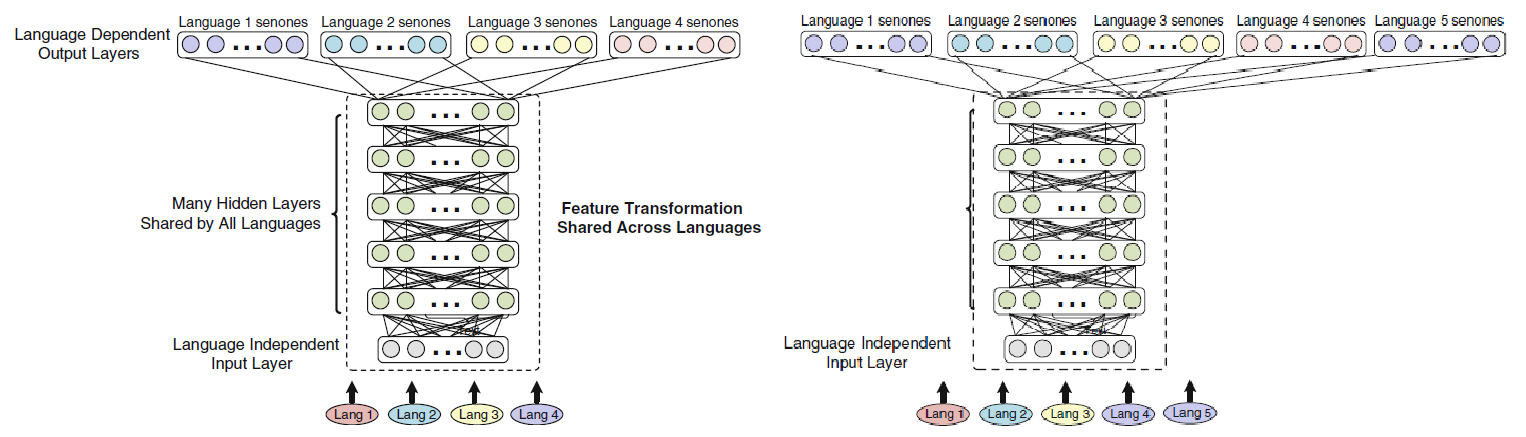
\includegraphics[width=1.0\linewidth]{images/shared_hidden_layer}
	\caption{Hinzufügen einer neuen Sprache  \cite{GonzalezDominguez.2015}} %Generelle
	\label{fig:topology}
\end{figure*}

Tatsächlich bringt dieser Ansatz eine Verbesserung gegenüber monolingualer Netzwerke. Ein Vergleich eines monolingualen Deep Neural Networks und eines multilingualen Deep Neural Networks ist in Tabelle (…) aufgeführt. Das monolinguale Netzwerk wurde hierbei nur mit jeweils einer der Sprachen französisch, deutsch, spanisch und italienisch trainiert, während das multilinguale System mit allen vier Sprachen trainiert wurde. Dabei wird die prozentuale Wortfehlerrate (Word error rate, WER) angegeben. Es ist zu erkennen, dass das multilinguale System das monolinguale in allen Sprachen übertrifft. Diese Verbesserung ist dem sprachübergreifenden Wissen zuzuschreiben [1]. Die Steigerungen sind zusätzlich relativ in Prozent angegeben. 

\begin{table*}[h!]
	\begin{tabular}{lllll}
		& FRA             & DEU           & ESP           & ITA             \\
		Test set size (words) & 40k             & 37k           & 18k           & 31k             \\
		Monolingual DNN WER   & 28.1\%          & 24.0\%        & 30.6\%        & 24.3\%          \\
		Mulitlingual DNN WER  & 27.1\% (-3.6\%) & 22.7 (-5.4\%) & 29.4 (-3.9\%) & 23.5\% (-3.3\%)
	\end{tabular}
	\centering
	\caption{Relative Wortfehlerrate}
	\label{my-label}
\end{table*}

In [2] wurden eine Reihe weiterer Versuche durchgeführt, um die Wirksamkeit eines solchen Systems zu evaluieren. Dabei wurde zwei verschiedene Zielsprachen verwendet. Zum einen das amerikanische Englisch, welches phonetisch nahe an den europäischen Sprachen der oben aufgeführten Tabelle liegt und Mandarin-Chinesisch, welches kaum Gemeinsamkeiten zu europäischen Sprachen bietet. Beim genauen Vorhersagen des gesprochenen kommt die Sprachidentifikation ins Spiel, durch welche Wörter ausgeschlossen werden können, die ebenfalls in Frage kommen, allerdings zum Wortschatz einer anderen Sprache gehören. Es wird hier mit statistischen Modellen gearbeitet, um anzugeben mit welcher Wahrscheinlichkeit welches Wort vorkommt oder aufeinander folgen können. Dabei gibt es verschiedene Lösungsansätze, um das gesprochene vorherzusagen. Oft werden tiefe neuronale Netze in Verbindung mit Hidden Markov-Modellen eingesetzt. Diese hybriden Systeme werden in der Literatur oft untersucht und beschrieben. Ein allerdings leistungsfähigeres Modell bieten die Recurrent Neural Networks. Diese Form von neuronalen Netzen werden heutzutage eingesetzt und erreichen hohe Genauigkeiten [1].


\section{Recurrent Neural Networks}
Im Bereich der Spracherkennung werden heutzutage sogenannte Recurrent Neural Networks eingesetzt, durch welche die Netzwerke ihre Erkennungsgenauigkeit erreichen. Das Modell dieser Netze erlaubt gerichtete, zyklische Verbindungen zwischen den Neuronen, wodurch es mit einem temporalen Verhalten ausgestattet wird. Recurrent Networks sind somit ideal zum Lernen von Datensequenzen geeignet. Sprache, also kontinuierliche Audiostreams fallen somit ebenfalls in das Anwendungsgebiet. Diese Form von neuronalen Netzen unterscheidet sich grundlegend von einem Feed Forward Deep Neural Network, da es nicht nur basierend auf Eingaben arbeitet, sondern auch auf interne Zustände zurückgreift. Diese internen Zustände speichern die vergangenen Informationen in der zeitlichen Reihenfolge, in welcher diese verarbeitet wurden. Somit ist ein Recurrent Neural Network dynamischer, als ein Deep Neural Network, welches lediglich eine statische Eingabe-Ausgabe-Transformation durchführt. Dabei wird eine Erweiterung des Backpropagation-Algorithmus eingesetzt. Die Backpropagation-Through-Time-Methode sorgt für das Berechnen der Gradienten. Diese werden im Gegensatz zum Standardalgorithmus über die einzelnen Zeitschritte aufsummiert. In dieser Erweiterung des Backpropagation, welche in Recurrent Neural Networks eingesetzt wird, werden lediglich die Parameter einzelnen Zeitschritte zwischen den Ebenen geteilt. In Abbildung (…) ist ein vereinfachtes Modell illustriert [1].

\begin{figure*}[h!]
	\centering
	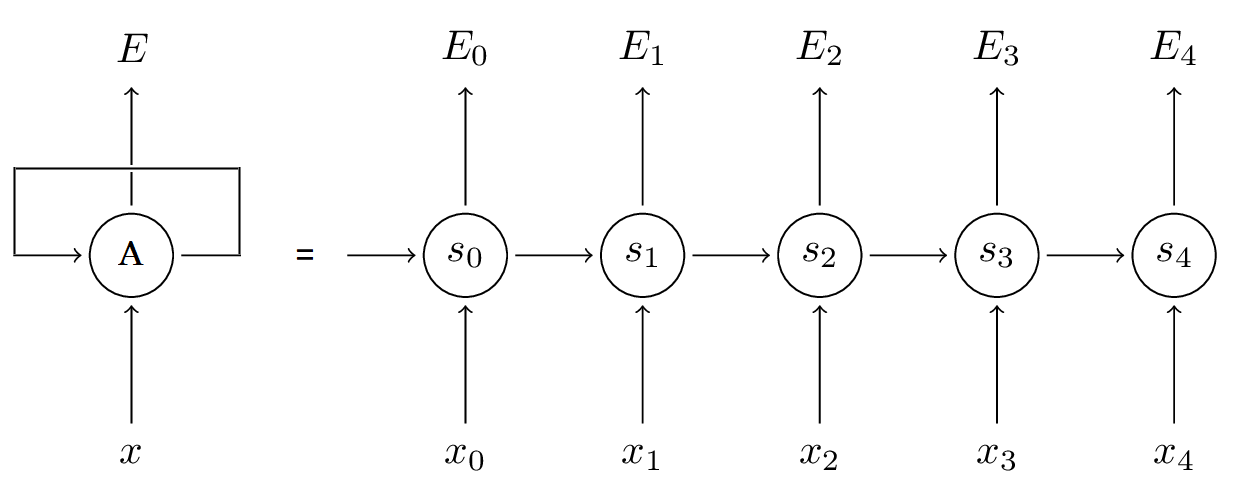
\includegraphics[width=0.8\linewidth]{images/rnn}
	\caption{Modell des Recurrent Neural Network  \cite{GonzalezDominguez.2015}} %Generelle
	\label{fig:topology}
\end{figure*}

Die Abbildung zeigt links ein Netzwerk A, welches über eine Rückkopplung verfügt. Dieses Netzwerk bekommt einen Input x und gibt einen Output bzw. Zustand E zurück. So kann die Information von einem Schritt zum nächsten gelangen. Das ausgerollte Netzwerk wird rechts daneben dargestellt. Es zeigt eine Folge von Iterationen. S bezeichnet den jeweiligen Schritt und E den entsprechenden Hidden State, welcher sich beim Eingeben von Daten zum Zeitpunkt s ergibt. Ein Recurrent Neural Network gibt somit nicht nur den Input an die nächste Iteration, sondern zusätzlich den daraus resultierenden Zustand. Vorhergehende Schritte beeinflussen so die darauf folgenden [1]. 
\\
Dies führt allerdings zu einem Problem. Dadurch, dass die Zustände immer weiter angepasst werden, verschwindet bzw. verschwimmt im Laufe der Zeit Information. Dies ist als Vanishing Gradient Problem bekannt und ergibt sich dadurch, dass Recurrent Neural Networks nicht in der Lage sind, auf Informationen zurückzugreifen, die weit in der Vergangenheit liegen. Der Kontext kann demnach bereits vergessen worden sein. Dieses Phänomen wird an Abbildung (...) deutlich. Das einmalige Anwenden der Sigmoidfunktion sorgt dafür, dass ein beliebiger Eingabewert zwischen -1 und 1 liegt. Wendet man die Funktion mehrmals an, flacht die Kurve ab und es kann keine Änderung mehr erkannt werden. Die Ausgaben streben alle den gleichen Wert an [https://deeplearning4j.org/lstm.html].

\begin{figure}[h!]
	\centering
	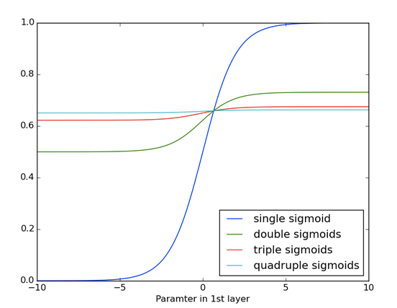
\includegraphics[width=1\linewidth]{images/vanishing_gradient}
	\caption{Modell des Recurrent Neural Network [deeplearning4j.org/lstm.html]  \cite{GonzalezDominguez.2015}} %Generelle
	\label{fig:topology}
\end{figure} 

So kann eine inkorrekte Vorhersage stattfinden. Aufgrund dessen wurden Long-Short-Term-Memory-Netzwerke entwickelt, die zur Lösung des Problems beitragen. Dabei werden Recurrent Neural Networks mit einer Speicherstruktur erweitert, was zur Namensgebung führt. Diese Netzwerke sind in der Lage, anhand des Kontextes zukünftige Wörter vorherzusagen und so ihre Genauigkeit zu erhöhen. Auch beim Lernen und Erkennen verrauschter, geräuschverzerrter oder hallender Aufnahmen bzw. schlechten Bedingungen beim bearbeiten der Merkmale kann diese Form von Netzwerken bessere Ergebnisse erzielen [1]. Die Verbesserte Genauigkeit wird in verschiedener Literatur belegt [1][3]. 
\\
Diese Form von Netzwerken erlauben die Erkennung zeitlich ausgedehnter Muster und von Zusammenhängen zeitlich getrennter Ereignisse. Somit eignen sie sich um Zeitreihen zu verarbeiten und vorherzusagen. Sogar, wenn zwischen wichtigen Ereignissen Verzögerungen liegen, die eine unbekannte Länge aufweisen. 
Die grundsätzliche Idee dabei ist es über elementweise Multiplikationen den Informationsfluss in dem Netzwerk zu steuern. Eine LSTM-Zelle kann als intelligente Netzwerkeinheit betrachtet werden, welche Informationen über einen Zeitraum speichern kann. Dies wird durch eine Gating-Struktur erreicht. Die Information passiert verschiedene Gatter. Es wird bestimmt, wann es wichtig ist, sich an eine vorhergehende Eingabe zu erinnern, wann sich die Zelle Informationen weiter merken oder diese vergessen sollte und wann sie die Information ausgibt. Ein Gatter ist dabei nichts weiter, als eine Reihe von Multiplikationen bzw. Matrixoperationen [1]. 
Das System ist somit in der Lage aus dem Kontext heraus genaue Vorhersagen zu treffen, wodurch die Spracherkennung präziser wird. Eine Darstellung einer LSTM-Zelle ist Abbildung (...) zu sehen. Der Input x wird zur Zeit t von mehreren Quellen in die Zelle eingespeist. Dabei wird x an alle Gatter übergeben. Jedes Gatter i (Input), f (Forget), c (Memory cell), o (Output) und h (Hidden vector bzw. der resultierende Zustand) haben dabei ihre eigene Gewichtungsfunktion [x4].   

\begin{figure}[h!]
	\centering
	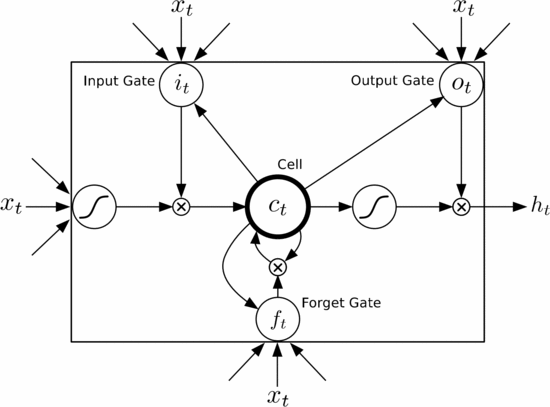
\includegraphics[width=1\linewidth]{images/lstm_cell}
	\caption{Modell des Recurrent Neural Network [deeplearning4j.org/lstm.html]  \cite{GonzalezDominguez.2015}} %Generelle
	\label{fig:topology}
\end{figure}  

Allerdings ist es selbst heute nicht möglich das Spracherkennungsproblem allgemein zu lösen. Spracherkennungssysteme werden somit nur für bestimmte Anwendungsfälle oder Szenarien konzipiert. Mit einer solchen Spezialisierung auf entsprechende Anwendungsgebiete können zum höhere Genauigkeiten erreicht werden. Zudem wird nicht so viel Rechenleistung und Speicher benötigt [4]. Vor allem bei der multilingualen Spracherkennung besteht die Schwierigkeit Gemeinsamkeiten verschiedener Sprachen zu nutzen, um Sprachen mit wenig Trainingsdaten mit einer ausreichenden Genauigkeit anzubieten. Es gilt die Sprachen zu finden, die zur besten Erkennungsleistung der neuen Sprache führen. Dabei müssen Beziehungen zwischen den Sprachen erkannt werden. Problematisch ist auch, dass gleiche Phoneme je nach Sprecher und Sprache variieren, was dazu führt, dass Phoneme nur im Kontext betrachtet werden (sogenannte Triphon-Zustände) [1]. Spracherkennungen verschiedener Unternehmen erreicht heute niedrige Wortfehlerraten (Google liegt bei 4,9\%), was auf die Menge von Trainingsmaterial zurückzuführen ist [x1] [x2] [x3]. In der Literatur wird außerdem gezeigt, dass verschiedene Kombinationen von tiefen neuronalen Netzen und LSTM-Netzwerken zu einer weiteren Verbesserung führen [x4]. 
	\section{Trainingsvorgang}

\subsection{Trainingsvorgang}
Der Trainingsvorgang basiert auf ein vollständig verbundenes mehrschichtiges Deep Learning-Netzwerk. Dieses Netzwerk aus Neuronen besteht aus drei Schichten:
\begin{description}
	\item Input-Schicht
	\item Hidden-Schicht 
	\item Output-Schicht
\end{description}
Die Input-Schicht stellt dabei die Eingangsdaten dar, welche als Trainingsmaterial für den Trainingsvorgang verwendet werden. Bei diesen Daten handelt es sich um Sprachaufnahmen. Bei Bedarf können diese Sprachaufnahmen dementsprechend vor-verarbeitet werden, wie zum Beispiel durch Einsatz von Filtern. Anschließend können die Daten in die Netztopologie beschriftet eingespeist werden. Eine Vorklassifizierung der Sprache führt zu erhöhten Erkennungsrate \cite{bishop.2006}. In der Hidden-Schicht geschieht das eigentlich Training, welches normalerweise durch die Sigmoid-Funktion aktiviert wird \cite{bishop.2006}. Die Schichten sind durch Kanten miteinander verbunden. Die Hier wird das Netz beginnend von der Input-Schicht bis Output-Schicht vollständig durchlaufen.
\begin{equation*}
sigm(x) :=\frac{ 1 }{1+e^{-x}  }
\label{normal}
\end{equation*}
Sobald die Output-Schicht erreicht ist, wird das Netz rückwärts durchlaufen. Dieses Verfahren wird auch Backpropagation-Algorithmus genannt und wird benötigt, um fehlerhafte Kantengewichte herauszufinden und anzupassen. Die Kantengewichte des Netzes werden anfangs mit null initialisiert, sodass die Kantengewichtungen korrigiert werden müssen. Die Ableitung der Sigmoid-Funktion kommt bei der Korrekturberechnung zum Einsatz \ref{ableitung}. Diese Funktion ist für eine geringe Datenmenge geeignet. Bei größeren Datenmengen entsteht ein Nachteil, welches sich auf die Wissensausprägung des Netzes auswirkt. Beim Rückwärts durchlaufen entsteht ein Wissensverlust \cite{bishop.2006}. Dieser Verlust wird durch das Maxima der Ableitung der verwendeten Funktion repräsentiert. Dieser kann bis zu 25 \% betragen. Der entstehende Verlust würde die Klassifizierungsrate des Trainingsmodels reduzieren, welches in Abbildung \ref{fig:features11.0} dargestellt ist \cite{Kulbear.2017}.
\begin{equation*}
sigm(x)':= \frac{ e^{x} }{(e^{x} +1)^2  }
\label{ableitung}
\end{equation*}

\begin{figure}[h!]
	\centering
	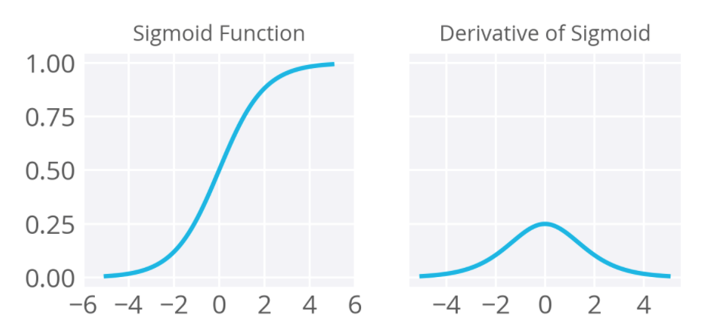
\includegraphics[width=1.0\linewidth]{images/sigmund}
	\caption{Darstellung der Sigmoid-Funktion und dessen Ableitung \cite{Kulbear.2017}} %Generelle
	\label{fig:features11.0}
\end{figure}
Anstelle der Sigmoid-Funktion wird in den modernsten Deep-Learning-Netzen Rectified linear Units ($ReLUs$) verwendet. Diese Funktion ist dem menschlichen Neuron am ähnlichsten und bringt zudem eine erhöhte Verarbeitungsgeschwindigkeit mit sich \cite{zeiler.2013}. Frameworks wie TensorFlow und TFLearn stellen diese Funktionalität bereits standardmäßig zur Verfügung, sodass diese Funktion nicht selber implementiert werden muss.
\begin{equation*}
y_{j} = ReLU(x_{j}) = max(0,x_{j}) 
\label{eq:ReLU}
%\caption{Rectiefied linear Units als Aktivierungsfunktion}
\end{equation*}
\begin{equation}
x_{ j } = b_{ j } + \sum{ }{ }{ x_{ ij } * y_{j}}
\label{eq:Gewichte}
%\caption{Berechnung der Output-Werte anhand der Gewichte und Neuronenwerte}
\end{equation}
Als Nächstes folgt die Output-Schicht, welches die Eingangsdaten dann zu den Klassen (Vorhersagen) zuordnet. Diese Schicht ist als Softlayer konfiguriert, welches die Klassen in eine eindimensionale Matrix kategorisiert. Eine Klasse steht für eine Sprache, die gelernt werden soll. Dabei ist die Matrix in dem Zahlenintervall $[0,1]$ normalisiert. Die endgültige Sprachidentifikation geschieht über normalisierte Werte, welches in Abbildung \ref{fig:soft} dargestellt wird. Die Werte können in Wahrscheinlichkeiten ausgedrückt werden, in dem diese mit dem Faktor 100 multipliziert werden \cite{Kulbear.2017}.
\begin{figure}[h!]
	\centering
	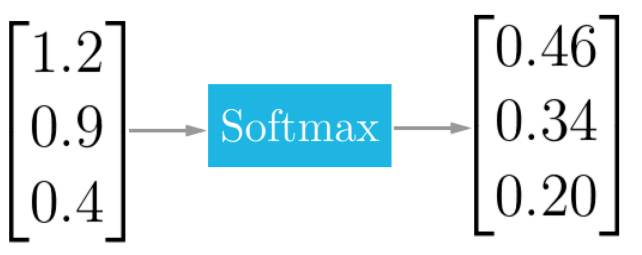
\includegraphics[width=0.7\linewidth]{images/softmax}
	\caption{Klassenzuordnung über Wahrscheinlichkeiten in der Softmax-Konfiguration \cite{Kulbear.2017}} %Generelle
	\label{fig:soft}
\end{figure}
 Die Vorhersagen der Output-Schicht geschieht durch die Funktion $p(j)$. Dabei steht der Index l für die jeweilige Klasse, also die Sprache, die gelernt werden soll.  
\begin{equation*}
p(j) := \frac{ exp(x_{j}) }{\sum_{l}{}{ exp(x_{l})} }
\label{eq:soft}
\end{equation*}
Für den vorhin erwähnten Backpropagation-Algorithmus wird ebenfalls eine Kostenfunktion benötigt. Diese geschieht durch Cross-Entropy-Loss-Funktion.
\begin{equation*}
C:= \sum_{l}{}{ t_{j} * log(p_{j})} 
\label{eq:back}
\end{equation*}
Diese Funktion misst die Abweichungen der Kantengewichte der Netztopologie und passt diese rückwirkend an. Der Cross-Entropy-Verlust nimmt zu, wenn der vorhergesagte Wert von der tatsächlichen Beschriftung (label) abweicht \cite{MLCheatsheet.2017}. Bei $t_{j}$ handelt es sich um die Klasse, für die der Verlust berechnet wird \cite{GonzalezDominguez.2015}.

\subsection{Netztopologie}
Die Netztopologie beschreibt die Infrastruktur des Netzes. Die Auswahl der Topologie bestimmt die Qualität des Trainingsvorgangs, d. h. die Anzahl der Neuronen. Eine zu geringe Anzahl führt zu einem niedrigen Klassifizierungsrate. Eine zu hohe Anzahl würde zu überhöhten Trainingsdauer führen. Aufgrund dessen fallen Topologien von Ansatz zu Ansatz unterschiedlich aus, welche unterschiedliche Spracherkennungsresultate liefern. In dieser Arbeit wird der Topologienvorschlag von Gonzales et al. betrachtet. Für die Eingangsdaten werden 40 Filterbanken verwendet. Diese werden benötigt, um die Daten samplen zu können. Als Input-Schicht wird werden 26 Knoten eingesetzt. Um unerwünschte Latenzzeiten der Frames zu vermeiden wird ein asymmetrischer Kontext verwendet. Die Hidden-Schicht beträgt vier Ebenen mit einer Gesamtzahl von 2560 Knoten. Die Output-Schicht enthält wie bereits erwähnt eine Softmax-Konfiguration, dessen Dimension der Anzahl der Zielsprachen entspricht. Dies ist bei der Erkennung von multilingualen Sprachen eine erforderliche Konfiguration.
 
%\begin{figure*}[h!]
%	\centering
%	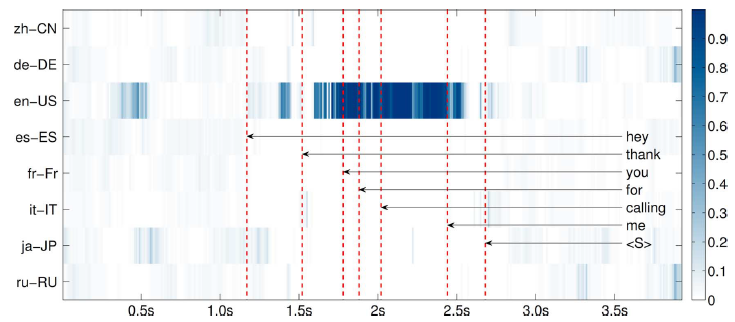
\includegraphics[width=1.0\linewidth]{images/Output}
%	\caption{Netztopologie zur  \cite{GonzalezDominguez.2015}} %Generelle
%	\label{fig:topology}
%\end{figure*}
\subsection{Verbesserung des Trainingsverfahrens durch Multitasking learning (MTL)}
 Bei maschinelles Lernen wird der Fokus gesetzt, bestimmte Metriken, wie beispielsweise Klassifizierungsgenauigkeit und Trainingsdauer, zu optimieren. Daraufhin wird das Modell soweit optimiert, bis die Leistung des Modells nicht mehr gesteigert werden kann \cite{Ruder.2017}. Das Lernen der einzelnen Sprachen läuft sequenziell ab. Hier setzt das Multitasking Learning (MTL) ein. Es werden mehrere Lernaufgaben gleichzeitig erledigt statt sequentiell, um das Trainingsvefahren effizienter zu gestalten. Das führt zu einer verbesserten Lerneffizienz und Vorhersagegenauigkeit. Im Klassifizierungskontext zielt MTL darauf ab, die Leistung mehrerer Klassifizierungsaufgaben zu verbessern, indem sie gemeinsam erlernt werden \cite{Lu_multitasklearning}. Ein Beispiel hierfür ist ein Spamfilter. Der Schlüssel zur erfolgreichen Anwendung von MTL besteht darin, dass die Aufgaben miteinander verknüpft werden können. Dies bedeutet nicht, dass die Aufgaben ähnlich sein müssen. Stattdessen bedeutet es, dass Aufgaben auf verschiedene Ebenen abstrahiert und geteilt werden. Wenn die Lernaufgaben tatsächlich ähnlich sind, können sie gemeinsam gelernt werden. Dabei kann das Wissen zwischen Aufgaben auf andere Lernaufgaben übertragen werden, welches die Trainingsdauer deutlich verkürzt. MTL ist vor allem dann nützlich, wenn die Größe des Trainingssatzes im Vergleich zur Modellgröße klein ist. Dabei wird grundsätzlich zwei Arten von MTL unterschieden: Hard parameter sharing und soft parameter sharing. \\ \\ Hard parameter sharing stellt das meist genutzte Art dar\cite{Ruder.2017}. Es wird normalerweise auf die Hidden-Schicht angewendet, indem die Aufgaben gemeinsam gelernt werden, während die spezifischen Aufgaben separat gelernt werden. Dies wird in Abbildung \ref{fig:hard} dargestellt. Dieser Ansatz reduziert das Risiko von overfitting erheblich. Je mehr Aufgaben gleichzeitig gelernt wird, desto mehr muss das Modell eine Repräsentation finden, die alle Aufgaben erfassen muss. Dadurch ist die Chance auf overfitting deutlich geringer \cite{Ruder.2017} \cite{Lu_multitasklearning}.
  \begin{figure}[h!]
 	\centering
 	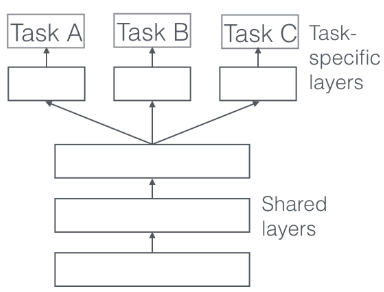
\includegraphics[width=0.8\linewidth]{images/hard}
 	\caption{Hard parameter sharing auf die Hidden-Schicht angewendet \cite{Kulbear.2017}.} %Generelle
 	\label{fig:hard}
 \end{figure}


	\section{Diskussion und Ausblick}
Die menschliche Sprache ist der natürlichste Weg etwas zu kommunizieren, so ist es nicht verwunderlich, dass das Interesse an Deep Learning-Ansätzen zur Spracherkennung und den damit verbundenen Anwendungen steigt. In dieser Arbeit wurde das Gegenstück zu den konventionellen, stochastischen Modellen beleuchtet - die Recurrent Neural Networks, mit der Erweiterung um die LSTM-Struktur. Dabei geht hervor, dass bei diesen Netzen die einzelnen Neuronen nicht isoliert betrachtet werden können. Vielmehr hängt deren Zustand und Aktivierung von den Aktivitäten anderer Neuronen bzw. Zellen ab. Vorhergehende Ereignissen beeinflussen den Zustand der folgenden. Durch die dynamische Rekursion und den Gattern wird ein Gedächtnis geschaffen, mit welchem sich die Netze an vergangene Zustände erinnern können und aufgrund dieser Erfahrungen genauere Vorhersagen treffen. Vor allem bei Datensequenzen ist dies hilfreich. Da die menschliche Sprache lediglich eine Sequenz von Tönen ist, eignet sich diese Form von Netzwerken ideal.\newline
Multilinguale Spracherkennungssysteme haben mit verschiedenen Problemen zu kämpfen. Dazu zählt beispielsweise die Ressourcenknappheit einiger Sprachen, wodurch die Kernidee eines solchen Systems vom gemeinsamen Verwenden der Phoneme ausgeht. Um erlerntes Wissen gemeinsam zu nutzen, wird ein solches System über das Multitask Learning trainiert. Es geht hervor, dass mit der multilingualen Spracherkennung bessere Ergebnisse erzielt werden, als mit der monolingualen Erkennung. Dies ist auf das gemeinsame Nutzen der Phoneme zurückzuführen. Heutige Genauigkeiten beim Erkennen von Sprachen erreichen die Wortfehlerrate eines Menschen. Somit ist das reine Verstehen bald nicht mehr das hauptsächliche Problem. Die Autoren sind der Meinung, dass eine natürliche Interaktion mit einem Spracherkennungssystem dennoch schwierig bleibt, solange das System keine Kenntnisse über seine Umwelt hat. Beispielsweise klingen im Deutschen die Worte 'Meer' und 'mehr' gleich, haben jedoch nichts gemeinsam. Diese Homophone lassen sich zwar verstehen, das Spracherkennungssystem erkennt allerdings nicht den Kontext und es könnte zu einer inkorrekten Vorhersage führen. Es bestehen auch weitere, zahlreiche limitierende Faktoren. Das Mapping von Wörtern und Sequenzen aus Phonemen braucht Linguistikexperten und stellt eine Herausforderung dar. Schließlich müssen sämtliche Phoneme der Sprache identifiziert werden. Auch der Stil beim Sprechen verändert sich ständig und ist nie gleich zwischen unterschiedlichen Sprechern. Gesprochene Wörter beeinflussen die Betonung der nächsten Worte.\newline
Die Zukunft im Bereich des maschinellen Lernens bleibt spannend. Wir sind überzeugt, dass in Zukunft fortschrittlichere Deep Learning-Architekturen für effektivere Spracherkennungssysteme entwickelt werden, die den hier diskutierten Netzwerken in vielerlei Hinsicht überlegen sind. Das Verständnis über die Struktur der Sprache, deren Dynamik und ihrer Repräsentation treiben den Forschungsfortschritt weiter voran. Ansätze, die in der Literatur zu finden sind, gehen davon aus, weitere Informationsquellen einzubeziehen, um die Qualität weiter zu verbessern. In diesem Zusammenhang wird in {\cite{Yu.2014}} das nutzen visueller Daten erwähnt. Dabei werden Merkmale aus interessanten Gesichtsregionen extrahiert. Da visuelle Informationen unabhängig von akustischem Rauschen sind, soll hier eine Verbesserung erzielt werden. Offen bleibt die Frage, welche Ansätze in Zukunft entwickelt werden, um die Interaktion mit Spracherkennungssystemen zu einem natürlichen Prozess zu machen. Da Maschinen die Welt nicht verstehen wie wir, ist es schwierig aus Tönen den gesamten Kontext abzuleiten. Weitere Forschungen können hier anknüpfen und sich mit potentiellen Möglichkeiten zur Lösung dieses Problems auseinandersetzen.

% Can use something like this to put references on a page
% by themselves when using endfloat and the captionsoff option.
\ifCLASSOPTIONcaptionsoff
  \newpage
\fi
	
	\bibliographystyle{IEEEtran}
	\bibliography{references}
	
	% that's all folks
\end{document}